\subsection{Ray tracing simulation}

\textbf{You will:}

\begin{itemize}
    \item simulate bending magnets
\end{itemize}



\textbf{Questions:}

\textbf{i)} Simulate the source for the ESRF1 bending magnet (the old storage ring, not longer existing) at a fixed energy (e.g.,. 8 keV). Use one mrad of horizontal divergence. Visualize the cross section (x,z), the divergence space (x’,z’), the phase spaces (x,x') and (z,z’). Visualize the top view (y,x). Make histograms of intensity (total, s-polarized and p-polarized) as a function of the vertical divergence. Plot also the degree of circular polarization (S3 component of the Stokes vector). 

\textbf{ii)} Change the source energy to 18 keV and compare the plot of intensity versus vertical divergence with the result at 8 keV. Verify that the radiation is more collimated. 

\textbf{Hints:} you may load the workspace {\tt bendingmagnet.ows}. 


\textbf{Answer}

Use the “Bending Magnet” widget,  click “Run shadow4/source” and display in the right panel using “Detailed Plot” the cross section (x,z), the divergence space (x’,z’),  and phase spaces  (x,x'), (z,z’).

\begin{figure}[H]
\label{fig:bm-fig1}
\caption{Rays in real space (X,Z), divergence space (X',Z'), phase space (X,X') along column 1, and phase space (Z,Z') along column 2,}
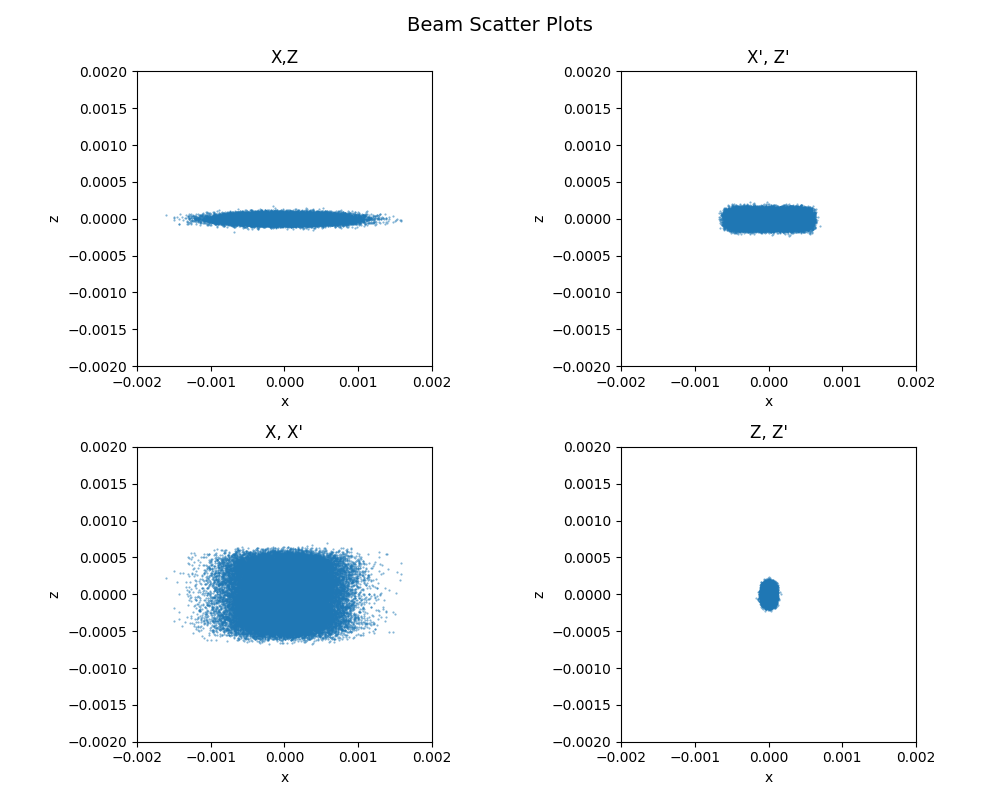
\includegraphics[width=0.8\textwidth]{bending-magnets/fig1.png}
\end{figure}

Another way is to plug a “Plot XY” widget and select the wanted coordinates for the plot. This can also be used to display the “top view” (y,x). 

Plug the “Histogram” widget to display histograms of intensity weighted by 23:Total Intensity, 24:s-polarized, 25: p-polarized, and 33: S3-Stokes or circular polarization. Although it is not possible to combine histograms in a single plot, it is always possible to prepare a simple script that performs customized plots, like the one included in the workspace that produces the outpur in figure 2.


\begin{figure}[H]
\label{fig:bm-fig2}
\caption{Histograms of the total intensity (weight column 23), S-polarization (weight column 24), P-polarization (weight column 25) and S3-Stokes (weight column 33), versus Z'.}
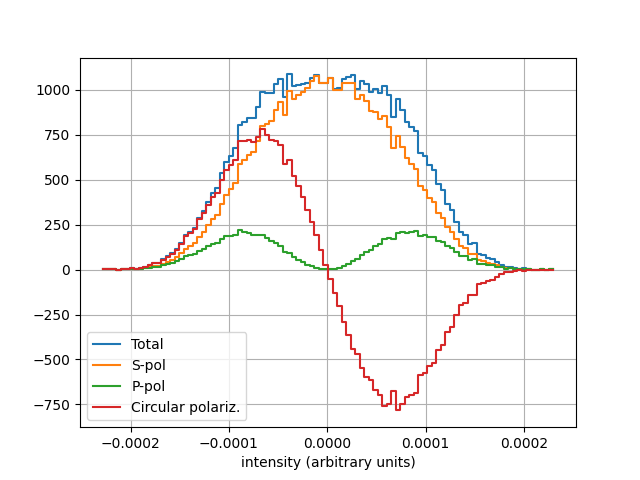
\includegraphics[width=0.6\textwidth]{bending-magnets/fig2.png}
\end{figure}


\begin{figure}[H]
\label{fig:bm-fig2}
\caption{Histograms of the total intensity vs Z' for emission at 8 and 18 keV.}
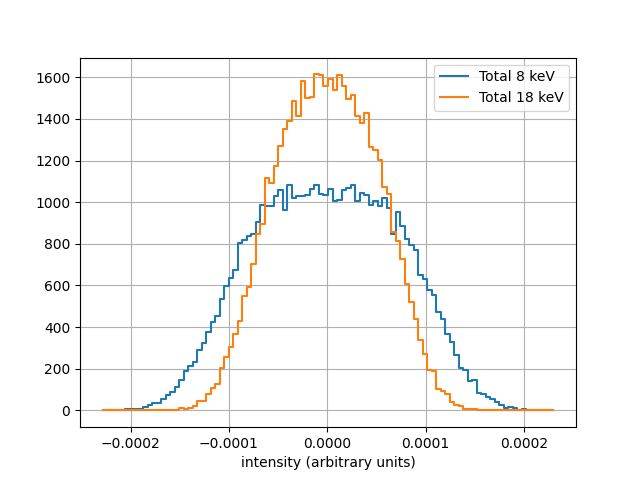
\includegraphics[width=0.6\textwidth]{bending-magnets/fig3.png}
\end{figure}